\section{Accumulator Concept}
\label{sec:accumulator-approach}



A simple concept, named \textit{accumulator}, has been proposed to improve \acrshort{mpi} communication during Jacobian matrix transfers preserving the current \acrshort{athlet}-\acrshort{nut} architecture and coupling.\\


The concept represents two arrays of length $2L$ where the first one, called \textit{accumulator}, is used for accumulation of Jacobian matrix elements, stored in the compressed coordinate sparse matrix format, till the critical array length equaled to $L = F \cdot N$; where $N$ is the size of the underlying Jacobian matrix and $F$ is a so-called capacity factor. Once the current array length of \textit{accumulator} exceeds its critical length, the accumulated data are moved to \textit{send buffer} by means of a simple swap of pointers, \textit{ACC\_PTR} and \textit{SEND\_BUFF\_PTR}, see Figure \ref{fig:accumulator-concept}. Having swapped the pointers and reset control variables, the accumulation process can be immediately resumed together with an immediate instantiation of the corresponding non-blocking broadcast operation with respect to \textit{send buffer} content.


\begin{figure}[!htpb]
  \centering
  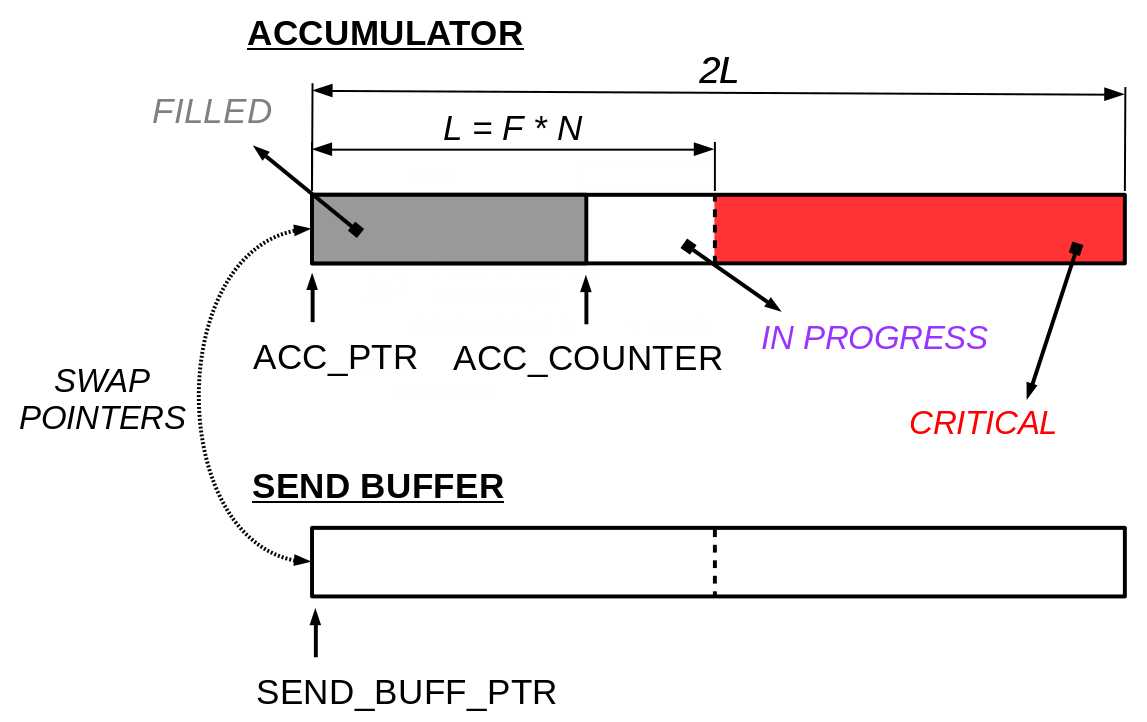
\includegraphics[width=0.8\textwidth]{figures/chapter-3/accumulator-concept.png}
  \caption{\textit{Accumulator} concept} \label{fig:accumulator-concept}
\end{figure}


The second array part of \textit{accumulator}, also called the critical part, is used for safe placement of data surplus without any extra program checks and manipulations. Additionally, this event triggers a signal for a regular pointer swap and, therefore, the subsequent non-blocking data transfer.\\


The factor $F$, depicted in Figure \ref{fig:accumulator-concept}, can be used by the user for two purposes. Mainly, it allows the user to adjust  \textit{send buffer} length $L$ till the point of saturation of physical interconnection bandwidth, see Figure \ref{fig:hw1-bandwidth} as an example, and thus achieve efficient resource utilization. Additionally, it reduces an amount of handshakes, i.e. an amount of resource acquisition requests, between \acrshort{nut} and a client. The default value of the factor is equal to 1, however, we insistently recommend to increase the value via the corresponding environment variable for small-sized problems and operation of \acrshort{nut} in a multi-client mode.


\begin{figure}[!htpb]
  \centering
  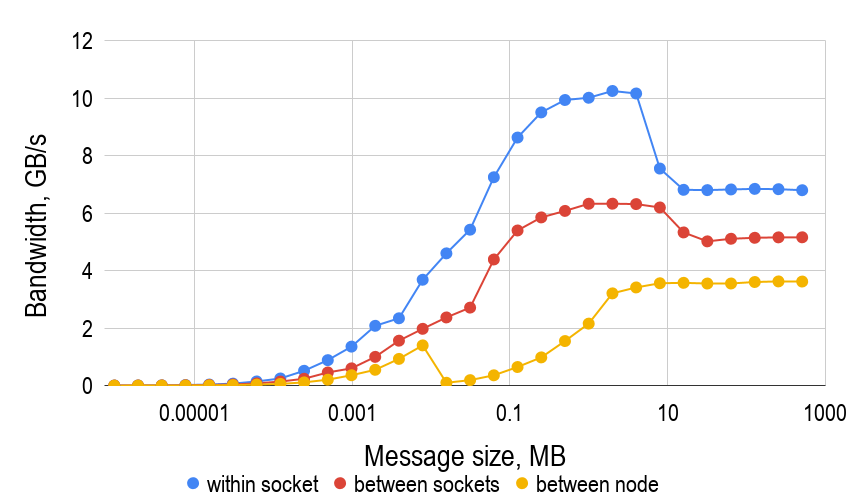
\includegraphics[width=0.8\textwidth]{figures/chapter-3/hw1-bandwidth.png}
  \caption{Technical characteristics of  \gls{hw1} hardware interconnection} \label{fig:hw1-bandwidth}
\end{figure}



Figure \ref{fig:accumulator-in-action} depicts an application of the \textit{accumulator} algorithm to the example represented in Figure \ref{fig:matrix-column-distribution} with the following parameters: $N = 100$ and $F = 1$. It can be clearly observed the algorithm reduces the number of transfers from 28 to 12. Additionally, the average column length, excluding the last one, jumps from 56 to 131. By and large, the algorithm allows to transform an original distribution shape to a more or less rectangular one which, in turn, allows to transfer a matrix in approximately equal chunks.\\



%\figpointer{\ref{fig:accumulator-in-action}}
\begin{figure}[!htpb]
\centering
	\begin{tabular}{cc}
		\subfloat[Before]{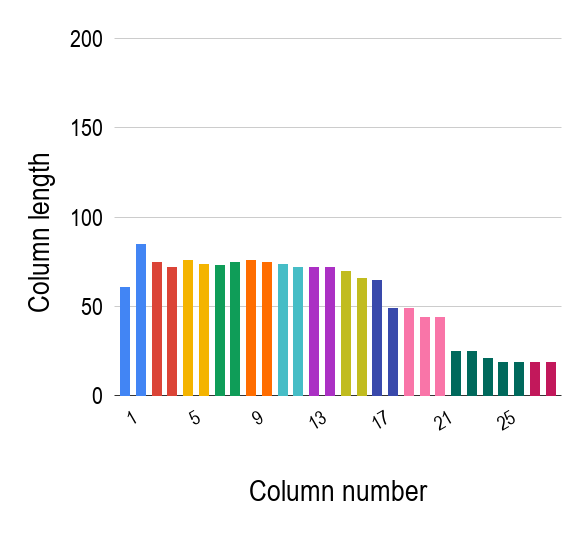
\includegraphics[width=0.48\textwidth]{figures/chapter-3/accumulation-before.png}} &
		\subfloat[After]{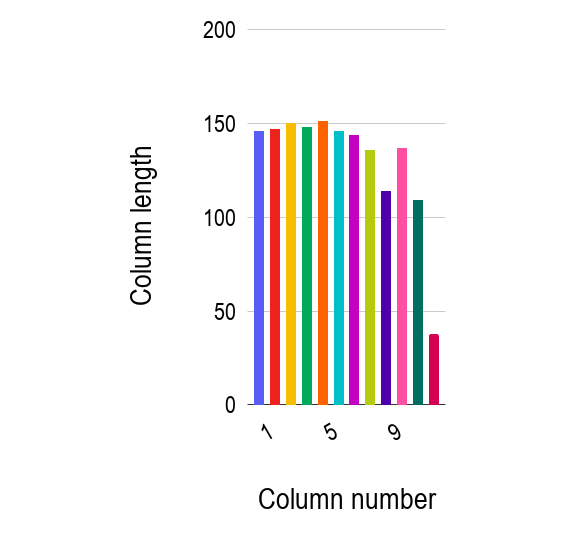
\includegraphics[width=0.48\textwidth]{figures/chapter-3/accumulation-after.png}} \\
	\end{tabular}
	\caption[An application of the \textit{accumulator} concept to the example depicted in Figure \ref{fig:matrix-column-distribution}]{An application of the \textit{accumulator} concept to the example depicted in Figure \ref{fig:matrix-column-distribution}, with $N=100$ and $F=1$}
	\label{fig:accumulator-in-action}
\end{figure}


Before \acrshort{athlet} can send a request to \acrshort{nut} to start solving Systems \ref{eq:athlet-10} it has to be certain that the entire Jacobian matrix has been transfered to the \acrshort{nut} side. For this reason, the last column transfer is done by means of the corresponding blocking \acrshort{mpi} operation. It means \acrshort{athlet} gets blocked only during the last column transfer and \acrshort{mpi} gives the execution control back only when the last piece of data has been successfully distributed among \acrshort{nut} processes.\\ 
